\section{Introduction}
\label{sec:introduction}


\par The objective of this laboratory assignment was to create a BandPass Filter using an OP-AMP. This filter should have a central frequency of 1 kHz and the gain should be 40dB at the central frequency. To implement this BandPass filter the following components were available: 
\begin{itemize}

\item One 741 OPAMP;
\item At most three 1 k$\Omega$ resistors;
\item At most three 10 k$\Omega$ resistors;
\item At most three 100 k$\Omega$ resistors;
\item At most three 220 nF capacitors;
\item At most three 1 uF capacitors.

\end{itemize} 


\par   
As in previous lab assignents, to determine the quality of the BandPass filter when compared to others, a merit classification system was created. This merit system took into account the cost of the components used, as well as the gain deviation and the central frequency deviation. The merit of the circuit will be determined according to the following equation: 
\begin {equation}
	 MERIT = \frac{1}{Cost*(Gain deviation + Central Frequency deviation + 10^(-6))  }   	
	\label{eq:i1}
\end{equation}

and the cost of the components are the following: cost of resistors = 1 monetary unit (MU) per k$\Omega$, cost of capacitors = 1 MU/uF
and cost of transistors = 0.1 MU per transistor. 

An image of the final circuit achieved in the presential lab class can be seen in the following \textbf{Figure~\ref{fig:circuit_t5}}.\par
\begin{figure}[h] \centering
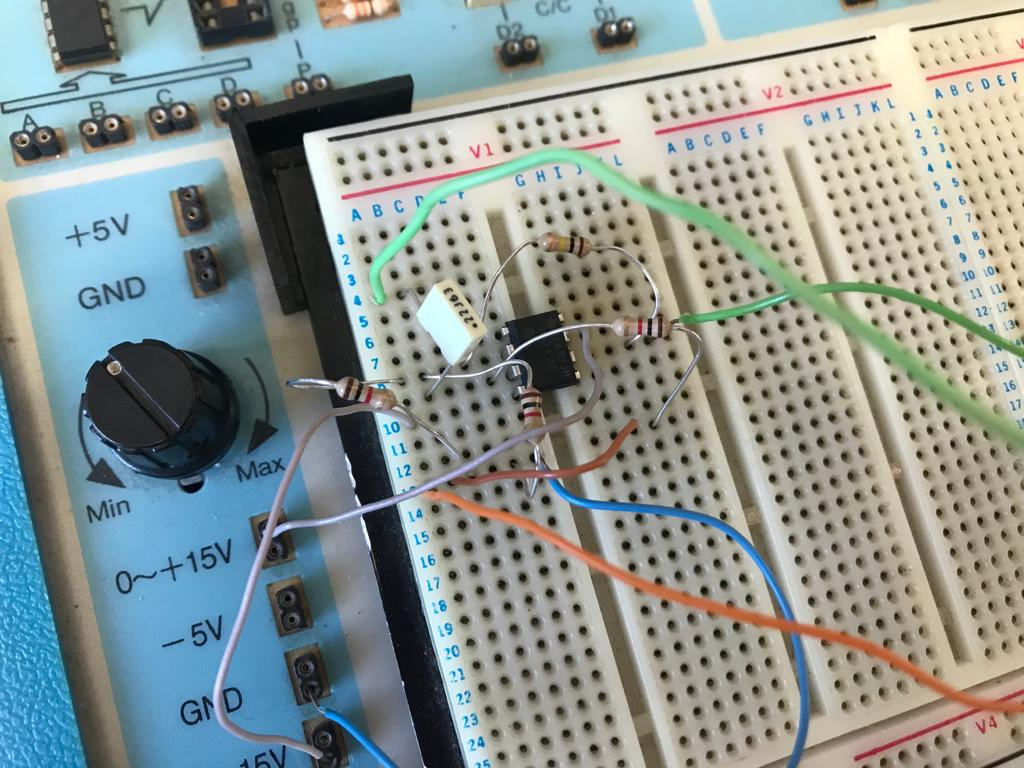
\includegraphics[width=0.6\linewidth]{circuit_t5.jpg}
%\vspace{-6cm}
\caption{Circuit in study}
\label{fig:circuit_t5}
\end{figure}


In Section~\ref{sec:analysis}, a theoretical analysis of the circuit is
presented. Here the circuit is analised using the suitable theoretical models studied in the class, in order to predict the gain and the input and output impedances at the central frequencies. To compute the frequency response of the gain, Vo(f)/Vi(f), here represented only as Vout, given the unitary input, and for the phase. This circuit was solved for a frequency vector in log scale with 10 points per decade, from 10Hz to 100MHz. 
In Section~\ref{sec:simulation}, the BandPass filter is analysed by
simulation using the program Ngspice. In Ngspice the OP-AMP model that was provided by the professor was used (the notorious 741 OP-AMP). The output voltage gain in the passband, the central frequency and the input and output impedances at this frequency were computed by simulation. 
In Section~\ref{sec:Presencial} the results from the work done at the laboratory is shown through some pictures, which allow for the determination of the gain and for an estimation of the central band frequency. The conclusions of this study are outlined in Section~\ref{sec:conclusion}, where the theoretical results obtained in Section~\ref{sec:analysis} are compared to the simulation results obtained in Section~\ref{sec:simulation}.





\pagebreak

